\chapter{Evolución molecular y filogenómica}\label{ch:b3:molecular-evolution}

En 1968 Motoo Kimura hizo una cuenta que inquietó a todo un campo. Al
comparar las hemoglobinas, los citocromos y otras proteínas de
mamíferos cuyos antepasados comunes databan los fósiles, halló que los
aminoácidos se habían sustituido a un ritmo de aproximadamente una
sustitución por sitio y por mil millones de años ---lo que, a lo largo
de un genoma de mamífero y de una generación, daba una sustitución
nueva fijada en la población cada dos años más o menos. Haldane había
demostrado una década antes que la selección natural puede fijar a lo
sumo una sustitución cada trescientas generaciones antes de que el
coste en descendencia perdida se vuelva impagable. La aritmética
dejaba una sola salida: la mayoría de los cambios que se acumulan en el
ADN no los impulsa la selección en absoluto, sino que son neutros y los
fija el azar en poblaciones finitas, a un ritmo que ---como muestra el
primer teorema de este capítulo--- es sencillamente el ritmo de
mutación. La \omterm{thm:b3:molecular-evolution:neutral}{teoría neutralista} se convirtió en la hipótesis nula de la
evolución molecular, la línea de base frente a la cual se detecta la
selección; el \omterm{prop:b3:molecular-evolution:clock}{reloj molecular} se convirtió en una manera de datar lo
que los fósiles no podían; y los genomas secuenciados desde entonces
han dado las herramientas para ver, gen a gen, dónde ha actuado la
selección, cómo nacen genes nuevos de los viejos y por qué el árbol de
un gen no siempre es el árbol de su especie.

\section{Deriva, mutación y el ritmo neutro}

\begin{theorem}[El ritmo neutro de sustitución]\label{thm:b3:molecular-evolution:neutral}
\index{teoría neutralista}\index{ritmo de sustitución}\index{probabilidad de fijación}\index{deriva genética}
En una población diploide de $N$ individuos, una mutación nueva sin
efecto sobre la eficacia biológica tiene una probabilidad $1/2N$ de
acabar reemplazando a todos los demás alelos (\emph{fijación}) y
$1 - 1/2N$ de perderse. Si cada una de las $2N$ copias del gen muta a un
ritmo $\mu$ por generación, surgen $2N\mu$ mutaciones neutras nuevas por
generación y, a la larga, el ritmo al que se acumulan las sustituciones
es
\[
k = 2N\mu\times\frac{1}{2N} = \mu :
\]
el \emph{\omterm{thm:b3:molecular-evolution:neutral}{ritmo de sustitución}} neutro es igual al ritmo de mutación, con
independencia del tamaño de la población. Una mutación destinada a
fijarse tarda en promedio $4N$ generaciones en conseguirlo, de modo que
las poblaciones grandes albergan más variación en tránsito, pero no la
fijan más deprisa. Para una mutación con ventaja selectiva $s$, la
fórmula de Kimura da la \omterm{thm:b3:molecular-evolution:neutral}{probabilidad de fijación}
\[
P(s) = \frac{1 - \mathrm{e}^{-2s}}{1 - \mathrm{e}^{-4Ns}} \approx 2s
\quad (4Ns \gg 1),
\]
de modo que una ventaja del \qty{1}{\%} se fija con una probabilidad de
alrededor del \qty{2}{\%} ---cuarenta veces la de una mutación neutra en
una población de dos mil, pero perdida aun así cuarenta y nueve veces de
cada cincuenta---; y una desventaja $s < 0$ con $4N|s| \gg 1$ no se fija
prácticamente nunca, mientras que una con $4N|s| \ll 1$ se comporta como
neutra: la selección solo ve lo que la deriva no anega, y la frontera
está en $|s| \sim
1/4N$ ---\emph{efectivamente neutra}.
\end{theorem}
\begin{proof}
Neutralidad: alguna copia presente hoy será la antepasada de toda la
población en un futuro lejano, y por simetría cada una de las $2N$
copias tiene la misma probabilidad de serlo; la nueva mutante es una
copia, de ahí $1/2N$. Ritmo: sustituciones por generación $=$
(mutaciones que surgen por generación) $\times$ (probabilidad de que
cada una se fije) $= 2N\mu/2N$. La fórmula de Kimura se sigue de la
aproximación por difusión al cambio de frecuencia alélica bajo deriva y
selección, admitida aquí; sus límites se comprueban directamente:
cuando $s \to 0$, $(2s)/(4Ns) = 1/2N$, el valor neutro; para
$4Ns \gg 1$ el denominador vale $1$ y el numerador $\approx 2s$. Tiempo
de fijación: la frecuencia de un alelo neutro hace un paseo aleatorio
con varianza $p(1-p)/2N$ por generación, y el tiempo esperado para
llegar a $1$ desde $1/2N$, condicionado a lograrlo, es de $4N$
generaciones (Kimura y Ohta, 1969), admitido.
\end{proof}

\begin{omfigure}
\begin{tikzpicture}
\begin{semilogyaxis}[
  width=0.62\linewidth, height=5.6cm,
  axis x line=bottom, axis y line=left,
  xmin=-4, xmax=8, ymin=0.00002, ymax=0.2,
  xlabel={$4Ns$ (coeficiente de selección escalado)}, ylabel={probabilidad de fijación},
  xlabel style={font=\small, at={(axis description cs:0.5,-0.12)}, anchor=north}, ylabel style={font=\small},
  tick label style={font=\small}, xtick={-4,-2,0,2,4,6,8}, ytick={0.0001,0.001,0.01,0.1}, yticklabels={$10^{-4}$,$10^{-3}$,$10^{-2}$,$10^{-1}$},
  clip=false,
]
\addplot[very thick, omDef, domain=-4:-0.05, samples=60] {(x/2000)/(1-exp(-x))};
\addplot[very thick, omDef, domain=0.05:8, samples=80] {(x/2000)/(1-exp(-x))};
\draw[dashed, gray] (axis cs:-4,0.0005) -- (axis cs:8,0.0005); \node[font=\scriptsize, gray, anchor=north west] at (axis cs:-3.9,0.00048) {neutra, $1/2N$};
\addplot[thick, omThm, dashed, domain=1:8, samples=2] {2*x/(4*1000)};
\node[font=\scriptsize, omThm, anchor=north west] at (axis cs:5,0.0012) {asíntota $2s$};
\node[font=\scriptsize, omDef, anchor=south east, align=right] at (axis cs:-0.2,0.02) {efectivamente neutra\\cuando $|4Ns| \lesssim 1$};
\node[font=\scriptsize, omDef, anchor=south west] at (axis cs:-3.9,0.0008) {deletérea: casi nunca se fija};
\end{semilogyaxis}
\end{tikzpicture}

{\small La \omterm{thm:b3:molecular-evolution:neutral}{probabilidad de fijación} de Kimura frente al coeficiente de
selección escalado, para $N = 1000$. Cerca de cero la curva pasa por el
valor neutro; a la derecha sube hacia $2s$; a la izquierda se despeña.
La selección actúa solo sobre lo que la deriva no puede esconder.}
\end{omfigure}

\begin{proof}[Evidencia]
Kimura (1968) y King y Jukes (1969) hicieron el razonamiento a partir
de los ritmos: el ritmo observado de sustitución de aminoácidos en las
proteínas de los mamíferos implicaba más sustituciones por generación
de las que permitía el coste de la selección de Haldane, de modo que la
mayoría tenía que ser neutra. Las predicciones de la teoría se
cumplieron después: los ritmos son máximos allí donde la función está
menos constreñida ---los sitios sinónimos, los intrones, los
seudogenes, la tercera posición del codón--- y mínimos en las \omterm{def:b3:chromatin-epigenetics:nucleosome}{histonas}
y en la ubiquitina, que cambian un residuo cada cien millones de años;
el nivel de variación dentro de una especie acompaña a la mutación y al
tamaño de la población; y el \omterm{thm:b3:molecular-evolution:neutral}{ritmo de sustitución} por año es
aproximadamente constante entre linajes de tamaños poblacionales muy
distintos, como exige la fórmula $k = \mu$ y como no hace una
explicación seleccionista. La polémica que siguió no la derribó: fijó
el ritmo neutro como la hipótesis nula frente a la cual se mide la
selección.
\end{proof}

\begin{omfigure}
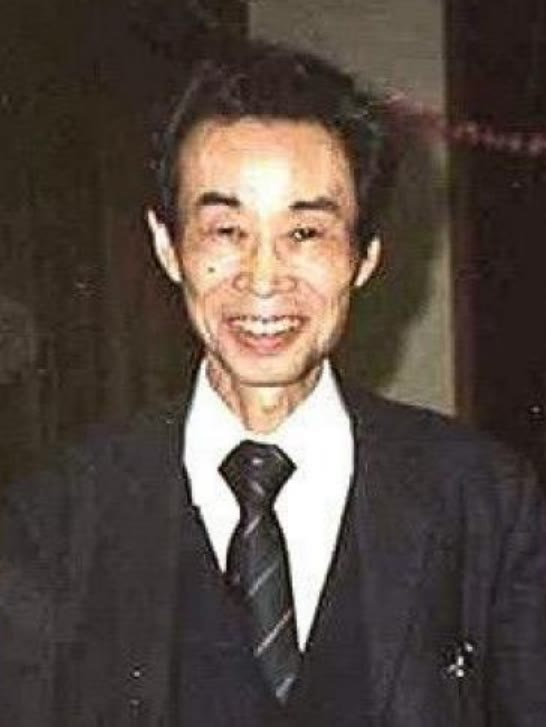
\includegraphics[width=0.34\linewidth]{images/book5/kimura.jpg}\hspace{0.05\linewidth}
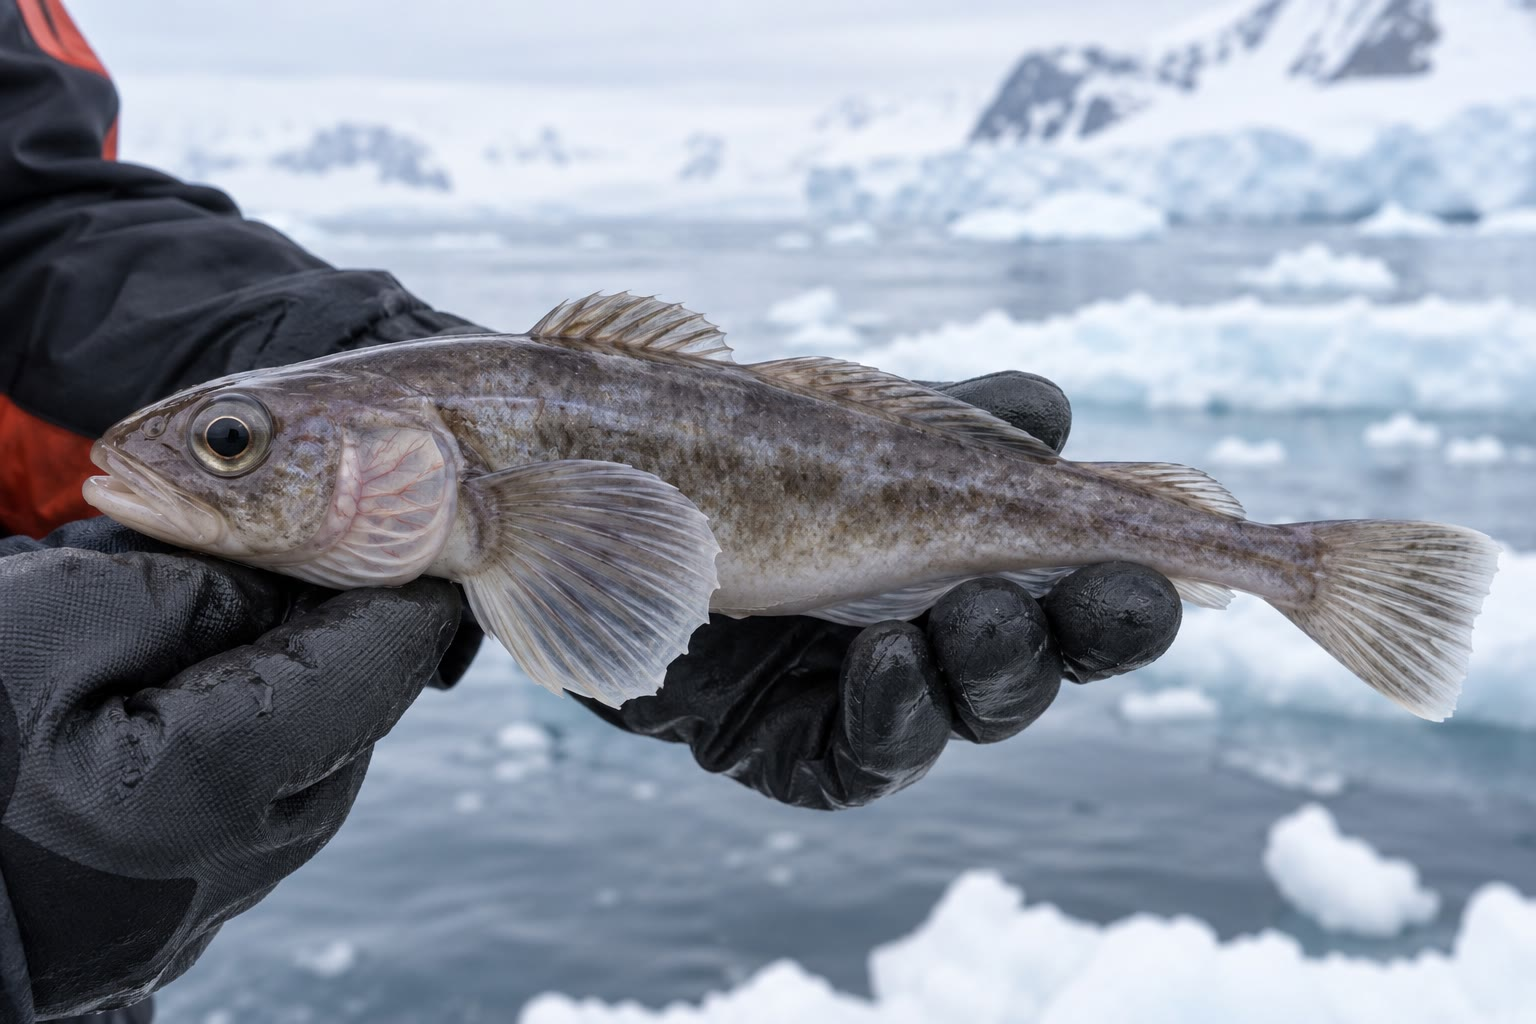
\includegraphics[width=0.5\linewidth]{images/book5/ai/b5-25-icefish.jpg}

{\small Izquierda: Motoo Kimura (1924--1994), que mostró que la mayor
parte del cambio molecular la fija el azar y al ritmo de mutación
(fotografía de 1986, CC BY 4.0). Derecha: un pez de hielo antártico,
cuya sangre evita congelarse gracias a una glucoproteína anticongelante
ensamblada, hace unos diez millones de años, a partir de un gen
duplicado de una enzima digestiva y de una serie de repeticiones.}
\end{omfigure}

\section{El reloj molecular}

\begin{proposition}[El reloj y sus irregularidades]\label{prop:b3:molecular-evolution:clock}
\index{reloj molecular}\index{calibración}\index{heterogeneidad de ritmos}\index{reloj relajado}\index{efecto del tiempo de generación}
Si las sustituciones se acumulan a un ritmo constante $k$ por sitio y
año en dos linajes que se separaron hace $T$ años, la fracción de
sitios en los que difieren es, para valores pequeños,
$d \approx 2kT$: la divergencia de dos secuencias es un \emph{\omterm{prop:b3:molecular-evolution:clock}{reloj
molecular}} (Zuckerkandl y Pauling, 1965), que puede \emph{calibrarse}
con una separación datada por fósiles y leerse después para
separaciones sin fósiles. El reloj es estocástico ---un proceso de
Poisson, de modo que $d$ tiene una varianza aproximadamente igual a su
media sobre un número fijo de sitios--- y es irregular de tres maneras
conocidas. Cada proteína tiene su propio ritmo, fijado por la fracción
de sus sitios a los que la función permite cambiar: los fibrinopéptidos
a \num{8}, la hemoglobina a \num{1}, el citocromo~$c$ a \num{0.3} y la
\omterm{def:b3:chromatin-epigenetics:nucleosome}{histona}~H4 a \num{0.01} sustituciones por sitio y por mil millones de
años. Los ritmos difieren entre linajes: como el ritmo neutro es $\mu$
por generación, los animales de generación corta (roedores) acumulan
más cambio al año que los de generación larga (primates, ballenas)
---el \emph{\omterm{prop:b3:molecular-evolution:clock}{efecto del tiempo de generación}}, compensado en parte
porque los ritmos de mutación por generación suben con la duración de
la generación. Y $d$ se satura: una vez que han cambiado muchos sitios,
los cambios siguientes caen en sitios ya cambiados, de modo que la
diferencia bruta ha de corregirse por impactos múltiples, como hacen
las distancias del capítulo del \omterm{def:b3:bioinformatics:alignment}{alineamiento}. Los \emph{\omterm{prop:b3:molecular-evolution:clock}{relojes
relajados}} modernos dejan que el ritmo varíe entre ramas dentro de un
modelo estadístico y se calibran con muchos fósiles a la vez; datan la
separación de humanos y chimpancés en seis o siete millones de años, la
de los órdenes de mamíferos placentarios cerca del final del Cretácico
y la de animales y hongos en el Precámbrico, con incertidumbres del
diez al veinte por ciento que proceden sobre todo de los fósiles.
\end{proposition}
\begin{proof}
Cada linaje acumula $kT$ sustituciones por sitio, de modo que la
diferencia entre ambos es $2kT$ allí donde los sitios no han recibido
dos impactos; un par datado por fósiles da $k = d/2T$. La varianza de
Poisson y los ritmos por proteína son los de Zuckerkandl y Pauling, los
de Dickerson (1971) y los ajustes de Kimura a conjuntos de proteínas de
vertebrados; la corrección por saturación es la fórmula de
Jukes--Cantor del capítulo del \omterm{def:b3:bioinformatics:alignment}{alineamiento}, $d_{\text{real}} =
-\tfrac{3}{4}\ln(1 - \tfrac{4}{3}p)$. La variación de ritmo entre
linajes se mostró con pruebas de ritmos relativos: con un grupo externo
$O$ y dos especies $A$ y $B$, las distancias $d_{AO} - d_{BO}$ deberían
ser cero bajo un reloj estricto, y no lo son para roedores frente a
primates.
\end{proof}

\begin{omfigure}
\begin{tikzpicture}
\begin{axis}[
  width=0.68\linewidth, height=5.8cm,
  axis x line=bottom, axis y line=left,
  xmin=0, xmax=600, ymin=0, ymax=110,
  xlabel={tiempo desde la divergencia (millones de años)}, ylabel={sustituciones por 100 sitios (corregidas)},
  xlabel style={font=\small, at={(axis description cs:0.5,-0.12)}, anchor=north}, ylabel style={font=\small},
  tick label style={font=\small}, xtick={0,100,200,300,400,500,600}, ytick={0,20,40,60,80,100},
  clip=false,
]
\addplot[very thick, omThm, domain=0:130, samples=2] {2*0.4*x};
\addplot[very thick, omDef, domain=0:600, samples=2] {2*0.09*x};
\addplot[very thick, omMeth!70!black, domain=0:600, samples=2] {2*0.03*x};
\addplot[very thick, omProp!80!black, domain=0:600, samples=2] {2*0.001*x};
\addplot[only marks, mark=*, mark size=1.8pt, omDef] coordinates {(80,13) (100,20) (300,52) (400,75) (450,80)};
\addplot[only marks, mark=*, mark size=1.8pt, omMeth!70!black] coordinates {(80,4) (300,17) (450,29) (550,33)};
\addplot[only marks, mark=*, mark size=1.8pt, omThm] coordinates {(30,22) (80,68) (100,80)};
\node[font=\scriptsize, omThm, anchor=west] at (axis cs:132,104) {fibrinopéptidos};
\node[font=\scriptsize, omDef, anchor=south east] at (axis cs:600,108) {hemoglobina};
\node[font=\scriptsize, omMeth!70!black, anchor=north west] at (axis cs:530,35) {citocromo $c$};
\node[font=\scriptsize, omProp!80!black, anchor=south east] at (axis cs:600,1.5) {histona H4};
\end{axis}
\end{tikzpicture}

{\small El \omterm{prop:b3:molecular-evolution:clock}{reloj molecular}, proteína a proteína. Cada una corre a su
propio ritmo, fijado por cuánto de la molécula deja libre la función
para cambiar: un fibrinopéptido, cortado y desechado cuando la sangre
coagula, cambia cientos de veces más deprisa que la \omterm{def:b3:chromatin-epigenetics:nucleosome}{histona} que empaqueta
el ADN.}
\end{omfigure}

\section{Leer la selección en las secuencias}

\begin{definition}[dN/dS]\label{def:b3:molecular-evolution:dnds}
\index{sustitución sinónima}\index{sustitución no sinónima}\index{razón dN/dS}\index{selección purificadora}\index{selección positiva}
En un gen codificante de proteína, una sustitución es \emph{sinónima}
si deja el aminoácido sin cambiar y \emph{no sinónima} si lo cambia.
Como el código genético deja cambiar en silencio la mayoría de las
terceras posiciones y algunas de las primeras, alrededor de una cuarta
parte de las mutaciones posibles de un gen típico son sinónimas. Sea
$d_{S}$ el número de sustituciones sinónimas por sitio sinónimo y
$d_{N}$ el de sustituciones no sinónimas por sitio no sinónimo,
corregidos ambos por impactos múltiples. Los cambios sinónimos son casi
neutros, de modo que $d_{S}$ estima $2\mu T$ ---el reloj---; y la razón
\[
\omega = \frac{d_{N}}{d_{S}}
\]
mide lo que la selección le ha hecho a la proteína: $\omega = 1$ si los
cambios de aminoácido son tan libres como los silenciosos (sin
restricción, como en un \omterm{def:b3:molecular-evolution:duplication}{seudogén}); $\omega < 1$ bajo \emph{selección
purificadora}, con la mayoría de los cambios eliminados ---el gen
típico tiene $\omega \approx 0.1$ a $0.2$, y las \omterm{def:b3:chromatin-epigenetics:nucleosome}{histonas} $0.001$---;
$\omega > 1$ bajo \emph{selección positiva}, con los cambios de
aminoácido favorecidos más deprisa de lo que permite la deriva sola
---el surco de unión al \omterm{def:b3:adaptive-immunity:lymphocytes}{antígeno} de las moléculas del MHC, las
proteínas de superficie de los \omterm{def:b3:virology:virus}{virus} en carrera de armamentos con los
\omterm{def:b3:adaptive-immunity:antibody}{anticuerpos}, las proteínas del espermatozoide y del óvulo en la
fecundación, y la lisozima de los rumiantes, reclutada para digerir
bacterias en el estómago. Calculado a lo largo de una rama de un árbol
o sitio a sitio, $\omega$ cartografía dónde y cuándo cambió la
selección una proteína en lugar del azar.
\end{definition}

\begin{omfigure}
\begin{tikzpicture}[every node/.style={font=\scriptsize}, >=stealth]
  \begin{axis}[
    width=0.52\linewidth, height=5.2cm,
    xbar, bar width=7pt, y=0.45cm,
    axis x line=bottom, axis y line=left,
    xmin=0.0005, xmax=5, xmode=log,
    xlabel={$\omega = d_{N}/d_{S}$},
    xlabel style={font=\small, at={(axis description cs:0.5,-0.12)}, anchor=north},
    symbolic y coords={histona H4, actina, insulina, gen tipico, citocromo $c$, seudogen, lisozima de rumiante, surco del MHC, envuelta del VIH},
    ytick=data, yticklabels={histona H4, actina, insulina, gen típico, citocromo $c$, seudogén, lisozima de rumiante, surco del MHC, envuelta del VIH},
    tick label style={font=\scriptsize},
    xtick={0.001,0.01,0.1,1}, xticklabels={0.001,0.01,0.1,1},
    clip=false,
  ]
  \addplot[fill=omDef!50, draw=omDef] coordinates {(0.002,histona H4) (0.01,actina) (0.09,insulina) (0.15,gen tipico) (0.05,citocromo $c$) (1,seudogen) (2.5,lisozima de rumiante) (3.5,surco del MHC) (4,envuelta del VIH)};
  \draw[dashed, thick, omThm] (axis cs:1,histona H4) -- (axis cs:1,envuelta del VIH);
  \node[omThm, anchor=south, font=\tiny] at (axis cs:1,envuelta del VIH) {$\omega = 1$: neutro};
  \node[anchor=east, font=\tiny, gray] at (axis cs:0.5,actina) {purificadora};
  \node[anchor=west, font=\tiny, gray] at (axis cs:1.6,insulina) {positiva};
  \end{axis}
\end{tikzpicture}

{\small Órdenes de magnitud de $\omega$. Casi todo gen se sitúa muy por
debajo de uno, con sus aminoácidos guardados por la \omterm{def:b3:molecular-evolution:dnds}{selección
purificadora}; un \omterm{def:b3:molecular-evolution:duplication}{seudogén} deriva en uno; los pocos que están por encima
de uno son las proteínas en carreras de armamentos o recién reclutadas
para un trabajo.}
\end{omfigure}

\begin{method}[Estimar $d_{N}/d_{S}$]\label{met:b3:molecular-evolution:method}
\index{alineamiento por codones}
(1) Alinéense las dos secuencias codificantes codón a codón (alinéense
las proteínas y trasládese después al ADN, de modo que ningún hueco
rompa la pauta de lectura). (2) Cuéntense para cada codón los
\emph{sitios} sinónimos y no sinónimos: cada una de sus tres posiciones
se puntúa por la fracción de cambios posibles que son silenciosos ---una
tercera posición cuádruplemente degenerada cuenta como un sitio
sinónimo, una posición en la que todo cambio altera el aminoácido como
un sitio no sinónimo, y una posición doblemente degenerada como un
tercio de uno y dos tercios del otro. Súmese sobre los codones: $S$
sitios sinónimos y $N$ no sinónimos, con $S + N = 3 \times$ codones. (3)
Cuéntense las \emph{diferencias} sinónimas y no sinónimas entre las
secuencias, resolviendo los codones que difieren en dos posiciones
promediando sobre los caminos posibles. (4) $p_{S} = $ diferencias$/S$,
$p_{N} = $ diferencias$/N$; corríjase cada uno por impactos múltiples
con Jukes--Cantor. (5) $\omega =
d_{N}/d_{S}$; contrástese $\omega \ne 1$ frente a la varianza muestral,
que es grande cuando $d_{S}$ es pequeño ---dos secuencias muy
emparentadas dan una razón poco fiable, y dos muy lejanas tienen un
$d_{S}$ saturado. (6) Para el dónde y el cuándo: ajústese $\omega$ por
rama de un árbol, o por sitio con una mezcla de clases de sitios, y
compruébese si una clase con $\omega > 1$ mejora el ajuste.
\end{method}

\section{Genes nuevos a partir de genes viejos}

\begin{definition}[Duplicación, familias y transferencia]\label{def:b3:molecular-evolution:duplication}
\index{duplicación génica}\index{familia génica}\index{neofuncionalización}\index{subfuncionalización}\index{seudogén}\index{transferencia horizontal de genes}
La mayoría de los genes nuevos son copias de genes viejos. Una
\emph{duplicación génica} ---por sobrecruzamiento desigual, por
retrotransposición o por la duplicación de un genoma entero, como
ocurrió dos veces en el origen de los vertebrados y otra vez en el
antepasado de los peces teleósteos y en muchos linajes vegetales---
deja dos \omterm{def:b3:genomics:comparative}{parálogos} donde había uno; los genes de especies
distintas descendientes de un solo gen ancestral son \omterm{def:b3:genomics:comparative}{ortólogos}.
El destino habitual de la copia es la decadencia: liberada de la
restricción ($\omega \to 1$), acumula un codón de parada o un
desplazamiento de pauta y se vuelve un \emph{seudogén}, de los cuales el
genoma humano lleva unos veinte mil. A veces sobreviven las dos: por
\emph{neofuncionalización}, cuando una copia adquiere una función nueva
mientras la otra conserva la vieja (la glucoproteína anticongelante del
pez de hielo, a partir de un gen de tripsinógeno; las opsinas roja y
verde de los primates, a partir de una duplicación de hace cuarenta
millones de años que dio la visión tricromática que describió el
volumen del Año~1; las cristalinas del cristalino, a partir de enzimas
metabólicas); o por \emph{subfuncionalización}, cuando cada copia
conserva parte de la expresión o de la actividad del antepasado, de modo
que hacen falta las dos. La duplicación repetida construye
\emph{familias génicas} ---las globinas, los grupos Hox del capítulo del
desarrollo, los mil genes de \omterm{def:b3:sensory-systems:chemical}{receptores olfativos} de un ratón, un tercio
de ellos seudogenes en el ser humano. La otra fuente de genes nuevos es
la \emph{transferencia horizontal}: las bacterias adquieren genes de
bacterias no emparentadas mediante \omterm{def:b3:genetic-engineering:tools}{plásmidos}, fagos y ADN libre, que es
como la resistencia a los \omterm{def:b3:bacteriology:antibiotics}{antibióticos} cruza especies en un hospital y
por qué la ``especie'' de una bacteria es un genoma central rodeado de
una nube cambiante; en los eucariotas la transferencia es más rara pero
real ---el T-DNA que \emph{\omterm{def:b3:genetic-engineering:plants}{Agrobacterium}} inserta en las plantas, los
genes bacterianos de los rotíferos bdeloideos y las antiguas
transferencias masivas que fueron la mitocondria y el cloroplasto. Allí
donde la transferencia es común, la historia de la vida es una red, y
el árbol dibujado a partir de un gen cualquiera es el árbol de ese gen.
\end{definition}

\begin{omfigure}
\begin{tikzpicture}[every node/.style={font=\scriptsize}, >=stealth]
  \node[draw, thick, rounded corners, fill=omDef!25, minimum width=1.8cm] (a) at (0,3) {gen ancestral};
  \node[draw, thick, rounded corners, fill=omDef!25, minimum width=1.2cm] (c1) at (-1.2,1.6) {copia 1};
  \node[draw, thick, rounded corners, fill=omDef!25, minimum width=1.2cm] (c2) at (1.2,1.6) {copia 2};
  \draw[->, thick] (a) -- (c1); \draw[->, thick] (a) -- (c2); \node[right, font=\tiny] at (0.9,2.4) {duplicación};
  \node[draw, thick, rounded corners, fill=gray!20, align=center] (ps) at (-3.6,-0.2) {seudogén\\$\omega \to 1$, luego\\codones de parada, decadencia};
  \node[draw, thick, rounded corners, fill=omThm!20, align=center] (neo) at (0,-0.2) {neofuncionalización\\una copia toma un trabajo nuevo\\(anticongelante, opsina roja/verde)};
  \node[draw, thick, rounded corners, fill=omMeth!25, align=center] (sub) at (3.9,-0.2) {subfuncionalización\\cada copia conserva parte\\de la expresión antigua};
  \draw[->, thick] (c1.south) -- (ps.north); \draw[->, thick] (c2.south) -- (neo.north); \draw[->, thick] (c2.south) -- (sub.north);
  \node[right, align=left, font=\tiny] at (5.9,1.6) {destino más común: pérdida en\\unos pocos millones de años ($\sim$\num{20000}\\seudogenes en el genoma humano)};
  \node[right, align=left, font=\tiny] at (5.9,0.4) {más raro: se conservan las dos, y una\\familia génica crece (globinas, Hox,\\\num{1000} receptores olfativos)};
  \node[right, align=left, font=\tiny] at (5.9,-0.8) {transferencia horizontal: un gen\\llega de otra especie ---\\rutina en las bacterias};
\end{tikzpicture}

{\small Los destinos de un gen duplicado. Liberada de la restricción, la
copia sobrante suele decaer; de vez en cuando la atrapa la selección
para una función nueva, o las dos copias se reparten entre ellas la
antigua.}
\end{omfigure}

\begin{proof}[Evidencia]
Ohno (1970) propuso la duplicación como fuente principal de genes
nuevos antes de que se hubiera secuenciado una sola familia; las
globinas lo confirmaron, con su árbol de $\alpha$, $\beta$, $\gamma$,
$\delta$, mioglobina y las globinas vegetales y bacterianas ajustando
las fechas de duplicación a la radiación de los vertebrados. Chen,
DeVries y Cheng (1997) mostraron que el gen anticongelante del pez de
hielo comparte su secuencia señal y sus secuencias flanqueantes con el
tripsinógeno y que las repeticiones anticongelantes surgieron por
expansión de un trozo de nueve nucleótidos que abarcaba una unión entre
intrón y exón: una proteína nueva a partir de las piezas sueltas de una
enzima digestiva, datada por el reloj en la congelación del océano
Antártico. Thornton y sus colaboradores (2006) reconstruyeron la
secuencia ancestral de los receptores de esteroides, sintetizaron la
proteína de cuatrocientos cincuenta millones de años y hallaron que
respondía solo a los estrógenos; dos sustituciones posteriores,
identificadas y puestas a prueba, cambiaron la preferencia de la copia
duplicada al cortisol ---un antepasado resucitado, y el camino entre él
y sus descendientes recorrido en el laboratorio.
\end{proof}

\section{Árboles de genes y árboles de especies}

\begin{proposition}[Clasificación incompleta de linajes]\label{prop:b3:molecular-evolution:ils}
\index{árbol de genes}\index{árbol de especies}\index{clasificación incompleta de linajes}\index{coalescente}\index{filogenómica}
El árbol de un gen no tiene por qué coincidir con el árbol de las
especies que lo llevan. Considérense tres especies con \omterm{prop:b3:molecular-evolution:ils}{árbol de
especies} $((A,B),C)$, con la separación $A$--$B$ precedida por una
población ancestral de tamaño $N$ que persistió $T$ generaciones antes
de la separación respecto de $C$. Dos copias del gen, una de $A$ y otra
de $B$, seguidas hacia atrás, \emph{coalescen} en un antepasado común a
un ritmo $1/2N$ por generación; la probabilidad de que aún no hayan
coalescido cuando entran en la población ancestral de las tres es
$\mathrm{e}^{-T/2N}$, y entonces los tres linajes coalescen en orden
aleatorio, de modo que dos tercios de las veces el árbol del gen agrupa
a $A$ o a $B$ con $C$. La probabilidad de que el árbol del gen
discrepe del \omterm{prop:b3:molecular-evolution:ils}{árbol de especies} es, por tanto,
\[
P_{\text{disc}} = \tfrac{2}{3}\,\mathrm{e}^{-T/2N} .
\]
Para humanos, chimpancés y gorilas, con un $T$ de unos cientos de miles
de generaciones y un $N$ cercano a \num{50000}, alrededor de un tercio
del genoma respalda un árbol en el que los humanos están más cerca de
los gorilas, o los chimpancés de los gorilas, que en el \omterm{prop:b3:molecular-evolution:ils}{árbol de
especies} ---y así se observa. Esta \emph{\omterm{prop:b3:molecular-evolution:ils}{clasificación incompleta de
linajes}}, junto con la duplicación y la pérdida y con la transferencia
horizontal, es la razón de que la \emph{filogenómica} infiera el \omterm{prop:b3:molecular-evolution:ils}{árbol
de especies} a partir de miles de \omterm{prop:b3:molecular-evolution:ils}{árboles de genes} bajo un modelo
coalescente, en lugar de concatenarlos y dibujar uno solo; permite
además estimar los propios tamaños de las poblaciones ancestrales a
partir de la fracción de árboles discordantes, y leer hibridaciones
antiguas (el ADN neandertal de los humanos modernos, el flujo génico
entre osos o entre mariposas) en árboles que discrepan en un sentido
que la deriva sola no produciría.
\end{proposition}
\begin{proof}
Dos linajes de una población diploide de $N$ eligen padres de entre $2N$
copias cada generación y comparten uno con probabilidad $1/2N$; a lo
largo de $T$ generaciones, la probabilidad de no hacerlo nunca es
$(1 - 1/2N)^{T} \approx
\mathrm{e}^{-T/2N}$. Los tres linajes que entran en la población
ancestral común son intercambiables, de modo que el primer par en
coalescer es cada uno de los tres pares con probabilidad $1/3$; solo el
par $(A,B)$ coincide con el \omterm{prop:b3:molecular-evolution:ils}{árbol de especies}, de ahí que $2/3$ de
estos casos sean discordantes. Ni el ritmo del coalescente ni la
intercambiabilidad dependen del gen, de modo que la fórmula vale para
cada locus neutro por separado, y la fracción de árboles discordantes
de un genoma estima $\mathrm{e}^{-T/2N}$.
\end{proof}

\begin{omfigure}
\begin{tikzpicture}[every node/.style={font=\scriptsize}, >=stealth]
  % species tree as thick grey tubes
  \fill[gray!25] (0,0) -- (0.9,0) -- (2.8,4.2) -- (1.9,4.2) -- cycle;
  \fill[gray!25] (1.6,0) -- (2.5,0) -- (2.8,4.2) -- (1.9,4.2) -- cycle;
  \fill[gray!25] (2.35,2.6) -- (3.15,2.6) -- (3.15,0) -- (3.9,0) -- (3.9,3.4) -- (3.2,5.6) -- (2.3,5.6) -- (1.9,4.2) -- (2.8,4.2) -- cycle;
  \node[below] at (0.45,0) {A}; \node[below] at (2.05,0) {B}; \node[below] at (3.5,0) {C};
  \node[above left, font=\tiny, gray!70!black] at (1.0,4.2) {separación A--B};
  \node[above left, font=\tiny, gray!70!black] at (1.0,5.6) {separación respecto de C};
  \draw[<->, gray!70!black] (-0.2,4.2) -- (-0.2,5.6) node[midway, left, font=\tiny, align=right] {$T$ generaciones,\\tamaño $N$};
  \draw[gray!50, dashed] (-0.2,4.2) -- (1.9,4.2); \draw[gray!50, dashed] (-0.2,5.6) -- (2.3,5.6);
  % concordant gene lineages (blue)
  \draw[very thick, omDef] (0.4,0) -- (2.1,3.8) -- (2.2,4.0); \draw[very thick, omDef] (2.0,0) -- (2.2,4.0); \draw[very thick, omDef] (2.2,4.0) -- (2.6,5.0); \draw[very thick, omDef] (3.5,0) -- (2.6,5.0);
  \node[right, align=left, omDef] at (4.6,4.6) {azul: A y B coalescen antes de\\la separación respecto de C --- concordante};
  % discordant lineages (red)
  \draw[very thick, omThm, dashed] (0.55,0) -- (2.35,4.2) -- (2.7,5.9); \draw[very thick, omThm, dashed] (2.15,0) -- (2.55,4.2) -- (2.9,5.3) -- (3.0,5.5); \draw[very thick, omThm, dashed] (3.65,0) -- (3.0,5.5); \draw[very thick, omThm, dashed] (3.0,5.5) -- (2.7,5.9);
  \node[right, align=left, omThm] at (4.6,3.2) {rojo: no logran coalescer en la\\población ancestral (probabilidad\\$\mathrm{e}^{-T/2N}$), y B se une después antes a C:\\el árbol del gen es $((B,C),A)$};
  \node[right, align=left] at (4.6,1.4) {$P_{\text{disc}} = \tfrac{2}{3}\,\mathrm{e}^{-T/2N}$:\\con $T = 2N$, uno de cada cuatro genes\\discrepa del árbol de especies};
\end{tikzpicture}

{\small \omterm{prop:b3:molecular-evolution:ils}{Árboles de genes} dentro de un \omterm{prop:b3:molecular-evolution:ils}{árbol de especies}. Los tubos
grises son poblaciones; las líneas son la ascendencia de un gen. Los
linajes que no logran encontrarse en la población ancestral corta entran
juntos en la más profunda y se emparejan al azar ---de modo que un
tercio del genoma de tres especies muy próximas cuenta una historia
distinta de la de las propias especies.}
\end{omfigure}

\begin{example}[Leer la historia de un genoma]\label{ex:b3:molecular-evolution:cichlids}
Las quinientas especies de cíclidos del lago Victoria surgieron en los
quince mil años transcurridos desde que el lago volvió a llenarse
---demasiado deprisa para que la mutación suministrara las diferencias
entre ellas. Sus genomas muestran cómo: las variantes que distinguen a
un pez que se alimenta del fondo de uno que raspa algas ya estaban
presentes como variación permanente en los peces de río que colonizaron
el lago, clasificadas y recombinadas, y aumentadas por hibridación
entre linajes; los genes de las opsinas se afinaron para aguas claras o
turbias mediante sustituciones que el $\omega$ de sus ramas muestra
haber sido seleccionadas; y los \omterm{prop:b3:molecular-evolution:ils}{árboles de genes} discrepan entre sí a lo
largo del genoma exactamente con el patrón que predicen la \omterm{prop:b3:molecular-evolution:ils}{clasificación
incompleta de linajes} y el flujo génico. Una radiación no es el origen
de genes nuevos, sino la redistribución de alelos viejos en
combinaciones nuevas bajo una selección nueva ---cosa que las secuencias
registran, alelo a alelo, si uno sabe leer un árbol que en realidad es
un bosque.
\end{example}

\begin{omfigure}
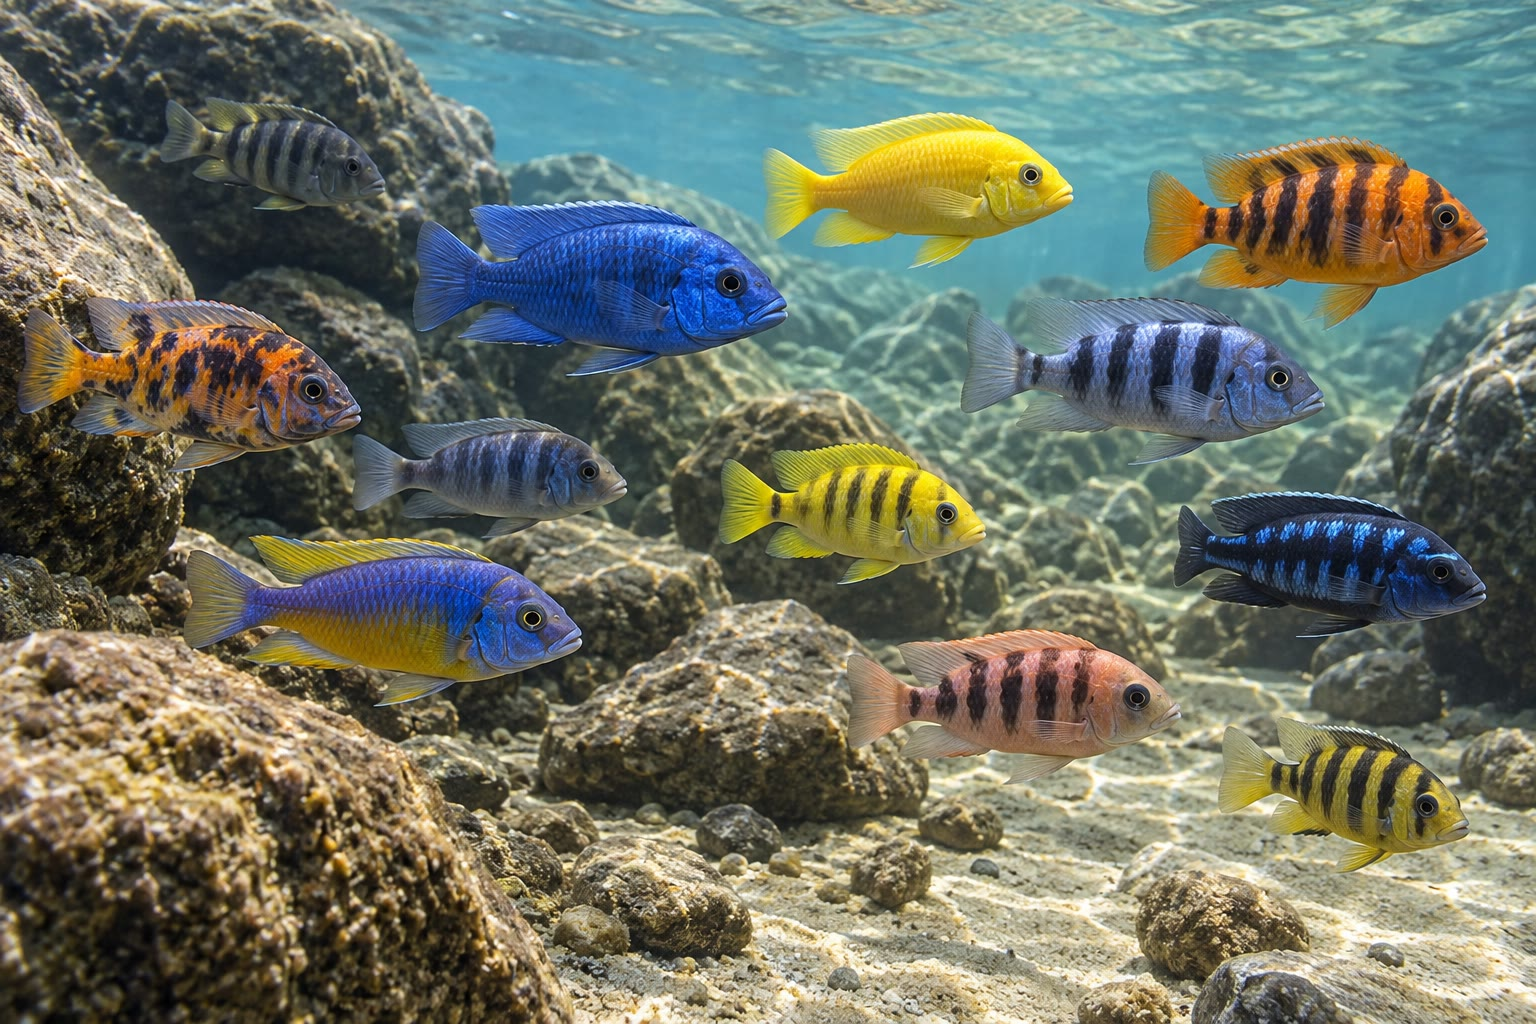
\includegraphics[width=0.6\linewidth]{images/book5/ai/b5-25-cichlids.jpg}

{\small Cíclidos de un lago africano: cientos de especies en unos pocos
miles de años, con sus diferencias sacadas en buena medida de la
variación que sus antepasados comunes ya llevaban.}
\end{omfigure}

\begin{remark}[El azar como línea de base]\label{rem:b3:molecular-evolution:remark}
La \omterm{thm:b3:molecular-evolution:neutral}{teoría neutralista} no afirma que la selección sea poco importante;
es un enunciado de lo que ocurre cuando la selección está ausente, lo
bastante preciso para contrastarse. Como el ritmo neutro es el ritmo de
mutación, la divergencia mide el tiempo; como el cambio neutro llena
los sitios que la selección deja libres, $\omega$ mide la restricción;
como los linajes neutros coalescen a un ritmo conocido, la discrepancia
de los \omterm{prop:b3:molecular-evolution:ils}{árboles de genes} mide el tamaño de poblaciones que nadie vio. La
selección es entonces lo que queda cuando se ha restado el azar ---un
gen con un $\omega$ por encima de uno, un barrido que ha vaciado de
variación una región, un árbol que discrepa en un sentido que la deriva
no puede explicar. El anticongelante del pez de hielo antártico, la
lisozima estomacal del rumiante y la tercera opsina del primate son las
excepciones halladas de este modo, y cada una es la historia de un gen
copiado y un trabajo nuevo. El resto del genoma es un reloj.
\end{remark}

\section{Ejercicios}

\begin{exercise}[$\star$]\label{exo:b3:molecular-evolution:1}
Enúnciese el ritmo neutro de sustitución y explíquese con palabras por
qué no depende del tamaño de la población.
\end{exercise}

\begin{exercise}[$\star$]\label{exo:b3:molecular-evolution:2}
Defínanse \omterm{def:b3:genomics:comparative}{ortólogo}, \omterm{def:b3:genomics:comparative}{parálogo} y \omterm{def:b3:molecular-evolution:duplication}{seudogén}, con un ejemplo de cada uno en
la familia de las globinas.
\end{exercise}

\begin{exercise}[$\star$]\label{exo:b3:molecular-evolution:3}
¿Qué mide $\omega = d_{N}/d_{S}$? Interprétense $\omega = 0.02$,
$\omega = 1.0$ y $\omega = 2.5$, y nómbrese un gen de cada clase.
\end{exercise}

\begin{exercise}[$\star$]\label{exo:b3:molecular-evolution:4}
¿Por qué concluyó Kimura que la mayoría de las sustituciones son
neutras? Reenúnciese el razonamiento con los números del comienzo del
capítulo.
\end{exercise}

\begin{exercise}[$\star\star$]\label{exo:b3:molecular-evolution:5}
$N = 5000$. Calcúlese la \omterm{thm:b3:molecular-evolution:neutral}{probabilidad de fijación} de una mutación nueva
con $s
= 0$, $s = 0.001$, $s = 0.01$ y $s = -0.001$, con la fórmula de Kimura, y
coméntese cuáles son efectivamente neutras.
\end{exercise}

\begin{exercise}[$\star\star$]\label{exo:b3:molecular-evolution:6}
Dos especies difieren en el \qty{12}{\%} de los sitios de un gen cuyo
ritmo neutro es de \qty{2e-9}{} por sitio y año. Estímese su tiempo de
divergencia con y sin la corrección de Jukes--Cantor. ¿Con qué
diferencia bruta alcanza la corrección un factor de dos?
\end{exercise}

\begin{exercise}[$\star\star$]\label{exo:b3:molecular-evolution:7}
Un gen de 300 codones tiene 700 sitios no sinónimos y 200 sinónimos.
Entre dos especies muestra 7 diferencias no sinónimas y 10 sinónimas.
Calcúlense $p_{N}$, $p_{S}$ y $\omega$ (sin corregir). ¿Qué régimen
selectivo? ¿Y si los recuentos fueran 35 y 10?
\end{exercise}

\begin{exercise}[$\star\star$]\label{exo:b3:molecular-evolution:8}
Las secuencias neutras de humano y chimpancé difieren en el
\qty{1.2}{\%}; la separación ocurrió hace \qty{6.5}{Myr} y el tiempo de
generación es de \qty{25}{yr}. Estímense el ritmo de mutación por sitio
y generación, y el número de mutaciones nuevas en un genoma diploide de
$6\times 10^{9}$ bases en cada generación.
\end{exercise}

\begin{exercise}[$\star\star$]\label{exo:b3:molecular-evolution:9}
Con $N = \num{50000}$ y $T = \num{100000}$ generaciones entre las dos
separaciones, calcúlese la fracción de \omterm{prop:b3:molecular-evolution:ils}{árboles de genes} discordantes
con el \omterm{prop:b3:molecular-evolution:ils}{árbol de especies} para humano, chimpancé y gorila. ¿Qué $T$ la
dejaría en el \qty{10}{\%}?
\end{exercise}

\begin{exercise}[$\star\star\star$]\label{exo:b3:molecular-evolution:10}
Muéstrese que la fórmula de Kimura se reduce a $1/2N$ cuando $s \to 0$
y a $2s$ para $4Ns \gg 1$, y que para $s < 0$ con $4N|s| \gg 1$ se
comporta como $2|s|\,\mathrm{e}^{-4N|s|}$. Estímese entonces cuán
deletérea ha de ser una mutación, en una población de $10^{4}$, para que
su \omterm{thm:b3:molecular-evolution:neutral}{probabilidad de fijación} quede cien veces por debajo de la neutra.
\end{exercise}

\begin{exercise}[$\star\star\star$]\label{exo:b3:molecular-evolution:11}
Una prueba de ritmos relativos: un grupo externo $O$ está a una
distancia corregida de $0.30$ del ratón y de $0.24$ del ser humano, y
el ratón y el ser humano distan $0.20$. Calcúlense las longitudes de las
ramas del ratón y del ser humano desde su separación (supóngase que el
punto de separación equidista de $O$ por los dos caminos) y su razón.
Con una generación de ratón de \qty{0.5}{yr} y una humana de
\qty{25}{yr}, ¿qué razón predeciría un reloj estricto por generación, y
qué dice la observación sobre los ritmos de mutación por generación?
\end{exercise}

\begin{exercise}[$\star\star\star$]\label{exo:b3:molecular-evolution:12}
Un gen duplicado queda liberado de la restricción ($\omega = 1$) a un
ritmo neutro $k = \qty{2e-9}{}$ por sitio y año. En una secuencia
codificante de 1000 bases, ¿cuántos años cabe esperar, a grandes rasgos,
hasta el primer codón de parada o desplazamiento de pauta (supóngase que
alrededor del \qty{4}{\%} de las mutaciones puntuales aleatorias de una
secuencia codificante crean un codón de parada, e ignórense las
inserciones y deleciones)? Compárese con el tiempo del que dispone la
selección para hallar una función nueva, y explíquese por qué la mayoría
de los duplicados muere.
\end{exercise}

\section{Problema: el ritmo del cambio}

\begin{problem}[{Problema de fin de semana --- la historia de un genoma
en números: el ritmo de mutación a partir de la divergencia entre humano
y chimpancé, la carga de sustitución de Kimura, las probabilidades de
fijación de las mutaciones seleccionadas, el $\omega$ de un gen a partir
de recuentos de codones, el reloj leído para una duplicación y la
discordancia de los árboles de genes entre los grandes simios, para
terminar en el ritmo de mutación, el $\omega$ del gen y la fracción
discordante}]
\label{pb:b3:molecular-evolution:1}
Datos: divergencia neutra humano--chimpancé $d = 0.012$; separación hace
\qty{6.5}{Myr}; generación \qty{25}{yr}; genoma diploide de $6\times
10^{9}$ bases, con un \qty{1.5}{\%} codificante. Población ancestral $N =
\num{50000}$. Gen: 400 codones, 920 sitios no sinónimos y 280 sinónimos;
diferencias humano--ratón, 46 no sinónimas y 84 sinónimas. Separación
humano--ratón, \qty{90}{Myr}. Globina: $\alpha$ y $\beta$ difieren en el
\qty{55}{\%} de los sitios de aminoácido (bruto); ritmo de la
hemoglobina, \num{1e-9} por sitio y año. Simios: $T$ entre las
separaciones del gorila y del chimpancé, \num{80000} generaciones.
Límite de Haldane: una sustitución seleccionada cada 300 generaciones.

\medskip
\noindent\textbf{Parte I --- El ritmo.}
\begin{enumerate}
  \item A partir de $d = 2kT$, calcúlese $k$ por sitio y año, y después
        $\mu$ por sitio y generación.
  \item Mutaciones nuevas por genoma diploide y generación, y cuántas de
        ellas caen en secuencia codificante.
  \item Sustituciones fijadas por generación en todo el genoma al ritmo
        neutro (la población fija $\mu$ por sitio y generación).
        Compárese con el límite de Haldane y sáquese la conclusión de
        Kimura.
  \item En una población de $N = \num{50000}$, ¿cuántas mutaciones
        neutras nuevas surgen por sitio y generación en toda la
        población, y qué fracción de ellas llegará a fijarse?
  \item ¿Cuánto tarda una mutación neutra destinada a fijarse, en
        generaciones y en años? Compárese con el tiempo transcurrido
        desde la separación humano--chimpancé.
  \item Explíquese por qué, pese a la pregunta~5, la divergencia entre
        dos especies mide el tiempo desde su separación y no el tiempo
        desde que se fijaron sus alelos.
\end{enumerate}

\medskip
\noindent\textbf{Parte II --- Las probabilidades de la selección.}
\begin{enumerate}[resume]
  \item \omterm{thm:b3:molecular-evolution:neutral}{Probabilidad de fijación} de una mutación neutra en
        $N = \num{50000}$, y de una con $s = 0.001$, $s = 0.01$ y
        $s = 0.1$.
  \item ¿Para qué $s$ vale $4Ns = 1$? Interprétese la frontera.
  \item Una mutación deletérea con $s = -0.001$: \omterm{thm:b3:molecular-evolution:neutral}{probabilidad de fijación}
        respecto de la neutra. ¿Y con $s = -10^{-5}$?
  \item Si una fracción $10^{-5}$ de las mutaciones nuevas de un gen son
        beneficiosas con $s = 0.01$ y el resto neutras, ¿qué fracción de
        las sustituciones de ese gen son adaptativas? Coméntese lo poco
        que se asoma la selección a la secuencia aun cuando actúa.
  \item Calcúlense $p_{N}$ y $p_{S}$ para el gen humano--ratón,
        corríjase cada uno con Jukes--Cantor y dese $\omega$.
  \item Interprétese $\omega$; y estímese el ritmo neutro que implica el
        $d_{S}$ del gen (por sitio y año) con el tiempo de separación.
        ¿Es coherente con la pregunta~1?
\end{enumerate}

\medskip
\noindent\textbf{Parte III --- Relojes y copias.}
\begin{enumerate}[resume]
  \item Corríjase por impactos múltiples la diferencia entre las
        globinas $\alpha$ y $\beta$ (úsese $d = -\ln(1 - p)$, la versión
        para proteínas con muchos estados) y dátese la duplicación con el
        ritmo de la hemoglobina.
  \item La fecha cae cerca del origen de los vertebrados con mandíbulas
        (\qtyrange{450}{500}{Myr}). ¿Qué permite tener cadenas $\alpha$ y
        $\beta$ separadas que no permite una sola cadena?
  \item Los fibrinopéptidos cambian a $8\times 10^{-9}$ por sitio y año.
        Dos especies se separaron hace \qty{40}{Myr}: ¿diferencia bruta
        esperada? ¿Por qué es inútil esta proteína para datar
        separaciones de \qty{500}{Myr}?
  \item La \omterm{def:b3:chromatin-epigenetics:nucleosome}{histona} H4 cambia a $10^{-11}$: ¿cuántas sustituciones en 100
        sitios a lo largo de \qty{1000}{Myr}? ¿Por qué es inútil para
        datar separaciones recientes?
  \item Un gen duplicado deriva con $\omega = 1$ desde el momento de la
        duplicación. Si el \qty{4}{\%} de las sustituciones de secuencia
        codificante crean codones de parada y el gen tiene 1200 sitios a
        un ritmo de $2\times
        10^{-9}$ por sitio y año, estímese el tiempo esperado hasta el
        primer codón de parada.
  \item ¿Por qué da una duplicación de genoma entero a los duplicados
        más posibilidades de sobrevivir que una sola duplicación en
        tándem?
\end{enumerate}

\medskip
\noindent\textbf{Parte IV --- Árboles dentro de árboles.}
\begin{enumerate}[resume]
  \item Probabilidad de que un linaje humano y uno de chimpancé no
        logren coalescer en las \num{80000} generaciones anteriores a la
        separación del gorila.
  \item Fracción de \omterm{prop:b3:molecular-evolution:ils}{árboles de genes} discordantes con el \omterm{prop:b3:molecular-evolution:ils}{árbol de
        especies}. Observada: alrededor del \qty{30}{\%}. ¿Es coherente?
  \item De los árboles discordantes, ¿qué fracción agrupa al humano con
        el gorila y qué fracción al chimpancé con el gorila? ¿Qué
        indicaría una desviación fuerte de la igualdad?
  \item Si la población ancestral hubiera sido de $N = \num{10000}$, ¿qué
        fracción discordante cabría esperar? ¿Qué dice, por tanto, la
        fracción observada sobre el número de nuestros antepasados?
  \item ¿Por qué concatenar mil genes en un solo \omterm{def:b3:bioinformatics:alignment}{alineamiento} da un
        árbol seguro pero posiblemente equivocado, y qué hace en su
        lugar un método coalescente?
  \item El ADN neandertal de los humanos no africanos ronda el
        \qty{2}{\%}, y los árboles que lo llevan agrupan a algunos
        europeos con los neandertales más a menudo que a los africanos.
        ¿Por qué no es esto una \omterm{prop:b3:molecular-evolution:ils}{clasificación incompleta de linajes}?
  \item Resúmase: $\mu$ (pregunta~1), el $\omega$ del gen (pregunta~11)
        y la fracción discordante (pregunta~20).
\end{enumerate}
\end{problem}
